% You will need to run LaTeX twice
\documentclass[mathserif]{beamer}
\usepackage[utf8]{inputenc}
\usepackage{lmodern}
\usepackage{ragged2e}
\usefonttheme{serif}
\usepackage{graphicx}
\usepackage{amsmath}
\usepackage{fancyvrb}
\usepackage{anyfontsize}
\usepackage{multicol}
\usepackage{wrapfig}
\usepackage{mflogo}
\usetheme{Luebeck}
\title{A presentation in \LaTeX{} beamer on \TeX{}/\LaTeX{}.}
\author{Jack Rosenthal}
\institute{CSM Linux Users Group}
\date{24 September 2015}
\font\bigtt=cmtt12 at 64pt
\beamertemplatenavigationsymbolsempty

\usepackage{xcolor}
\usepackage{tikz}
\usetikzlibrary{decorations.pathreplacing,calc}
\usepackage{listings}

\definecolor{maincs}{RGB}{255,0,0}
\definecolor{secondarycs}{RGB}{255,179,246}

\lstset{
    language=[LaTeX]TeX,
    xleftmargin=2cm,
    escapeinside={*@}{@*},
    basicstyle=\ttfamily\small,
    columns=fullflexible,
    breaklines=true,
    texcsstyle=*\color{maincs},
    texcs={documentclass,begin,end,chapter,section,subsection,label,alpha,part},
    moretexcs=[2]{usepackage,input},
    texcsstyle=*[2]{\color{secondarycs!80!black}},
}

\newcommand{\tikzmark}[1]{%
\tikz[baseline=-0.55ex,overlay,remember picture] \node[inner sep=0pt,] (#1) {\vphantom{T}};}

\newcommand{\braced}[3]{%
    \begin{tikzpicture}[overlay,remember picture]
        \draw [thick,decorate,decoration={brace,raise=1ex,amplitude=4pt},blue] (#2.south west-|T1.south west) -- node[anchor=west,left,xshift=-1.8ex,text=olive]{#3} (#1.north west-|T1.south west);
    \end{tikzpicture}
}

\begin{document}
\begin{frame}
    \titlepage
\end{frame}
\title{\TeX{}/\LaTeX}
\begin{frame}
    \titlepage
\end{frame}
\title{\texttt{lugtex.tex}}
\begin{frame}
    \titlepage
\end{frame}
\begin{frame}
    \frametitle{What are these things you say?}
    \centering
    \only<2,22>{
\includegraphics[width=\linewidth]{texfz}}
    \only<3>{
\includegraphics[width=\linewidth]{digital}}
    \only<4>{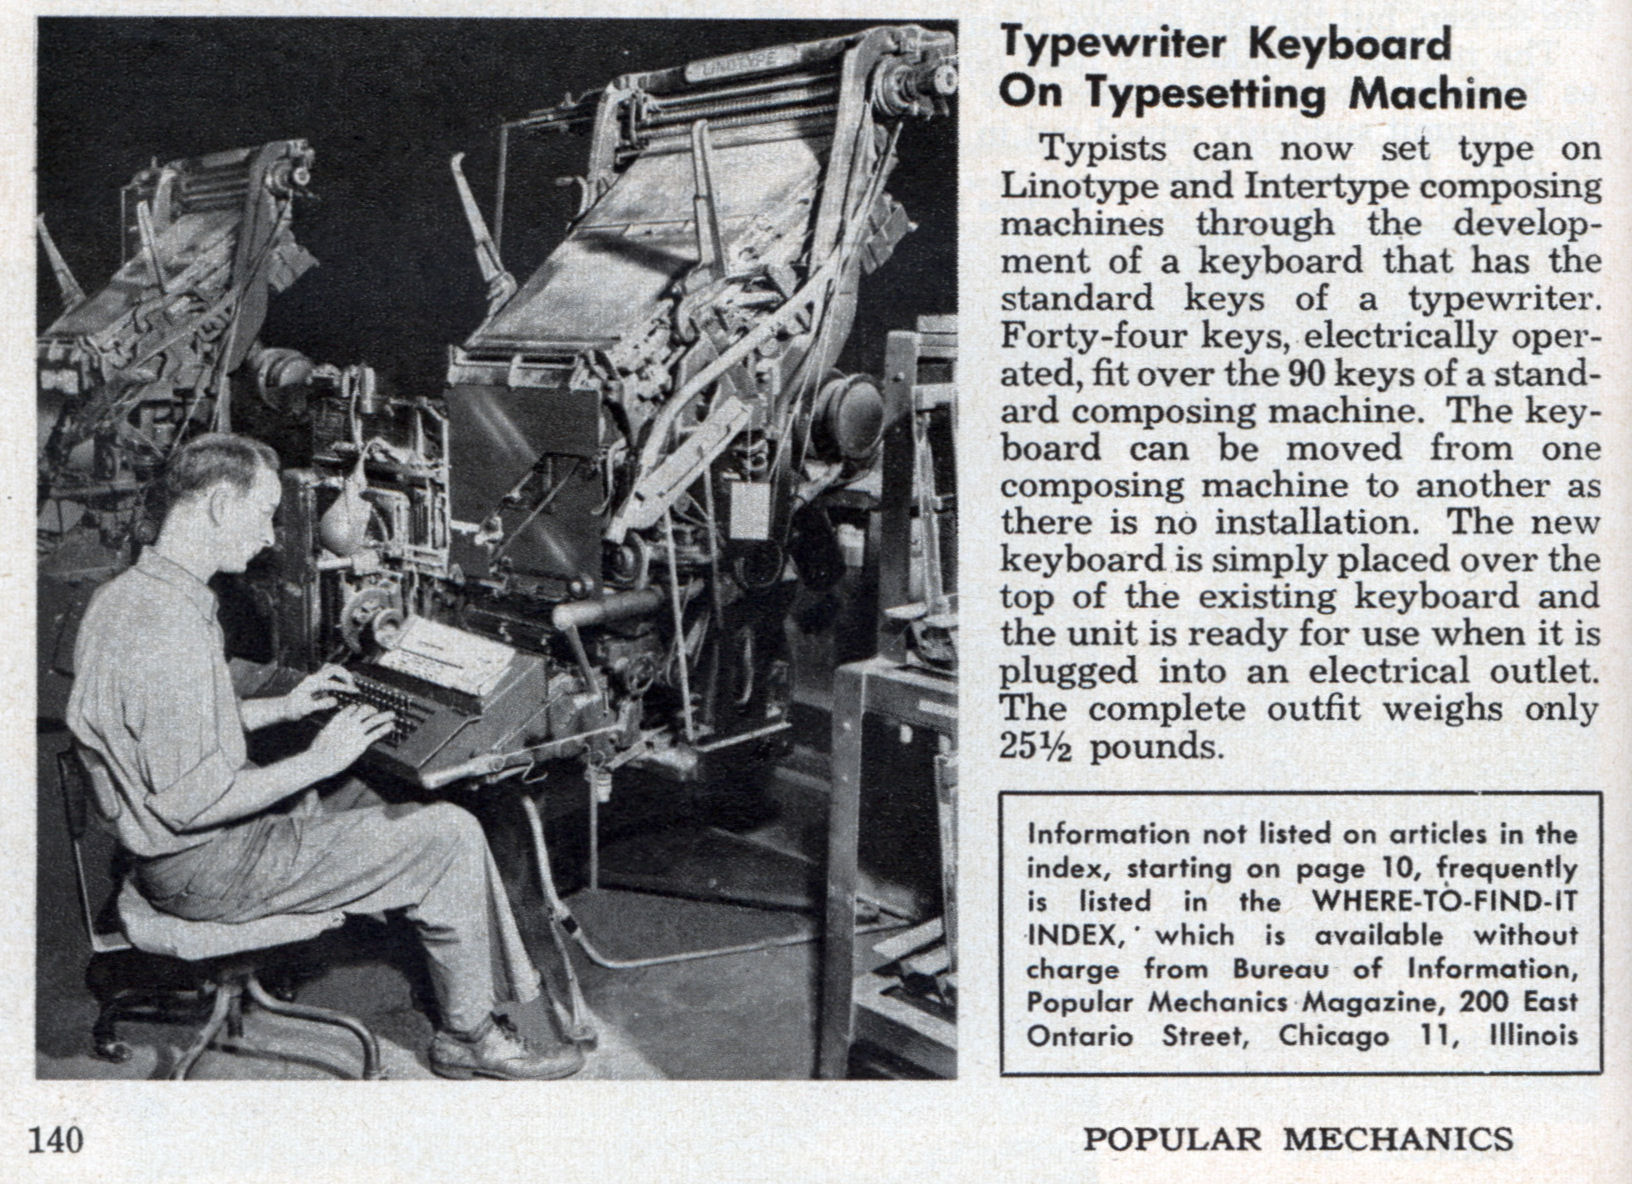
\includegraphics[width=\linewidth]{typesetter}}
    \only<5,20>{
\includegraphics[width=\linewidth]{system}}
    \only<6>{
\includegraphics[width=\linewidth]{design}}
    \only<7>{
\includegraphics[width=\linewidth]{by}}
    \only<8>{
\includegraphics[height=0.7\linewidth]{donald}}
    \only<9>{
\includegraphics[width=\linewidth]{E}}
    \only<10>{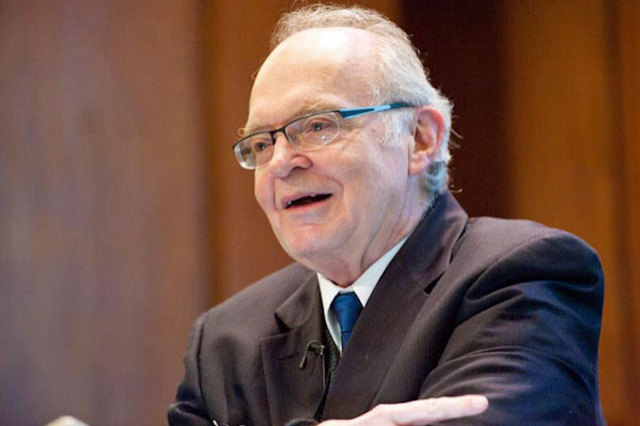
\includegraphics[width=\linewidth]{knuth}}
    \only<11>{\bigtt for (;;)}
    \only<12>{
\includegraphics[width=\linewidth]{create}}
    \only<13>{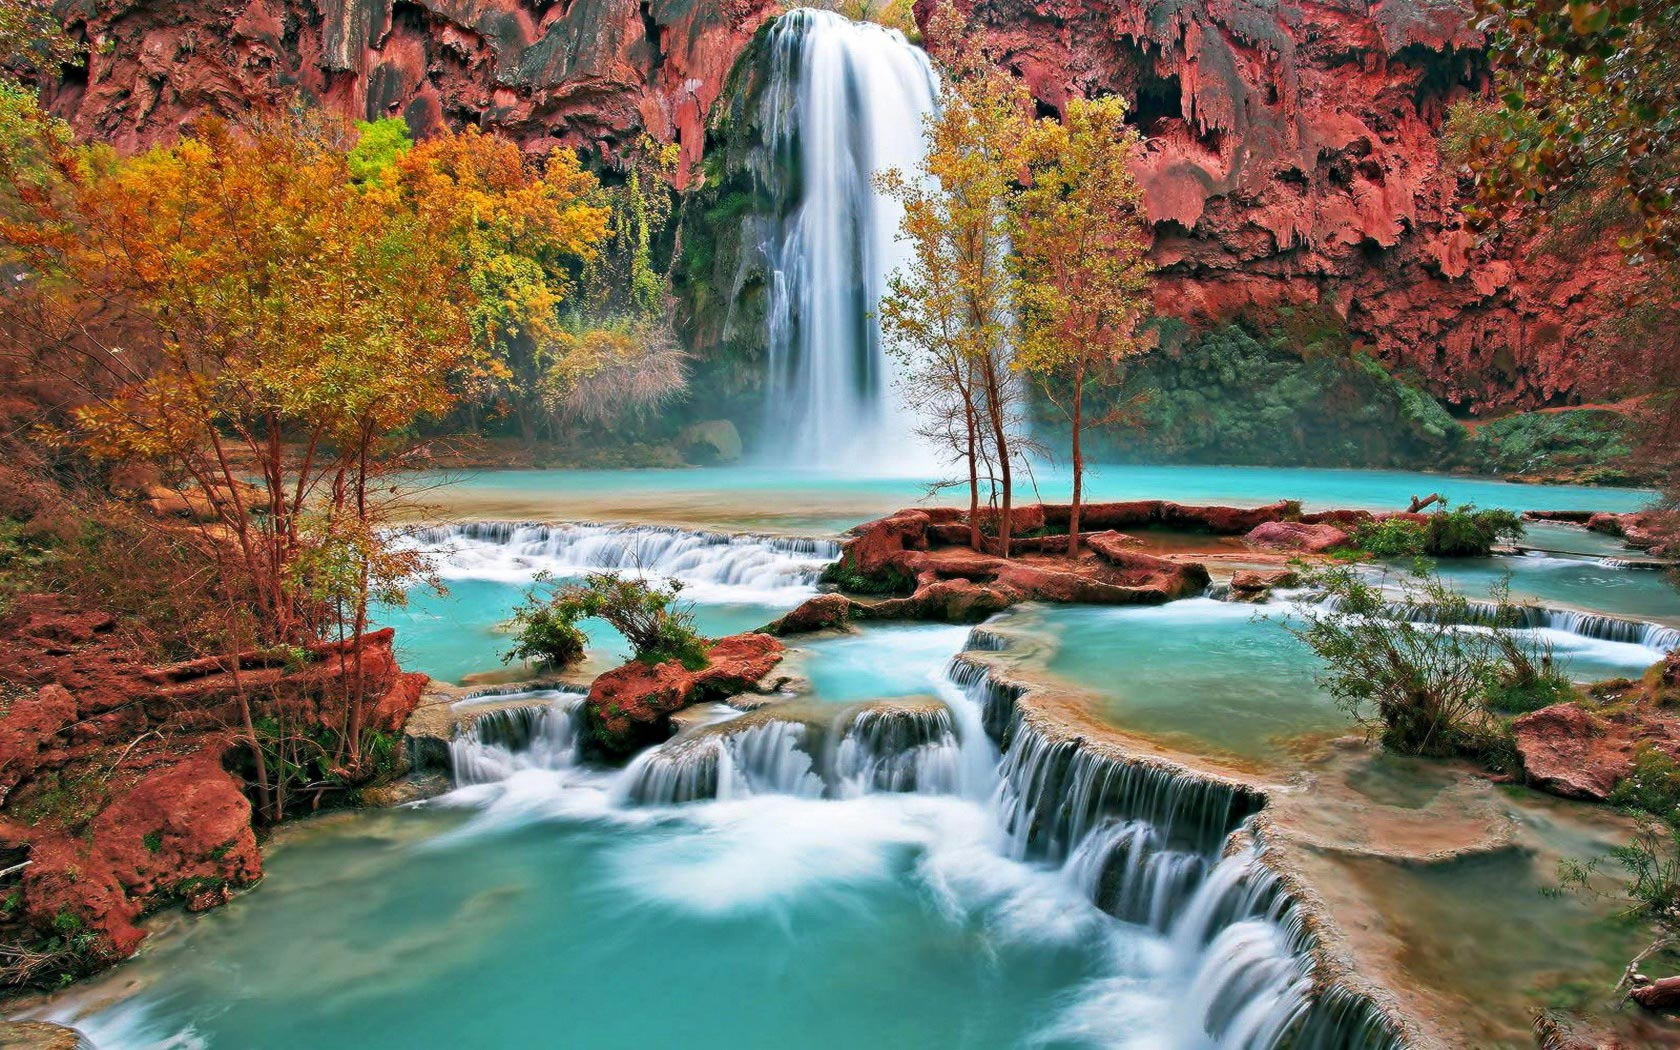
\includegraphics[width=\linewidth]{beautiful}}
    \only<14>{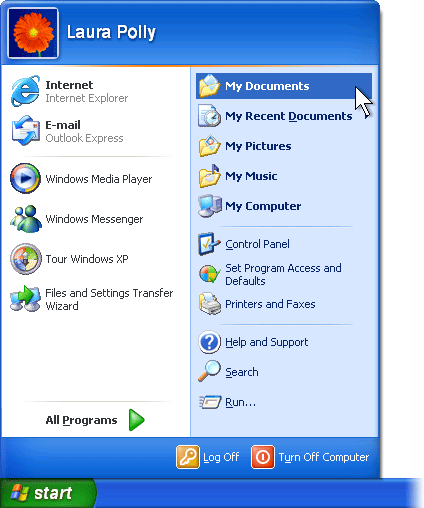
\includegraphics[width=\linewidth]{documents}}
    \only<15>{
\includegraphics[width=\linewidth]{and}}
    \only<16>{
\includegraphics[height=0.7\paperheight]{texbook}}
    \only<17>{
\includegraphics[width=0.7\paperheight]{latexlion}}
    \only<18>{\includegraphics[width=0.8\linewidth]{/home/jack/Dropbox/classes/cs/261/final/definition/definition.pdf}}
    \only<19>{
\includegraphics[width=\linewidth]{preparation}}
    \only<21>{
\includegraphics[width=\linewidth]{written}}
\end{frame}

\begin{frame}
    \frametitle{The Name of the Game}
    \only<1>{\begin{block}{From the \TeX book}
            \justifying
            English words like `technology' stem from a Greek root beginning with
            the letters $\tau\epsilon\chi\ldots$; and this same Greek word means
            \textsl{art} as well as technology...

            \medskip
            Insiders pronounce the $\chi$ of \TeX\ as a Greek chi, not as an `x',
            so that \TeX\ rhymes with the word blecchhh... When you say it
            correctly to your computer, the terminal may become slightly moist.
    \end{block}}
    \only<2>{\begin{block}{From \LaTeX : A Document Preparation System}
            \justifying
            One of the hardest things about \LaTeX\ is deciding how to pronounce it. This is
            also one of the few things I'm not going to tell you about \LaTeX, since
            pronunciation is best determined by usage, not fiat. \TeX\ is usually pronounced
            teck, making lah-teck, and lay-teck the logical choices.
    \end{block}}
\end{frame}

\begin{frame}
    \frametitle{Typesetting vs. Ordinary Typing}
    \begin{itemize}[<+->]
        \item Typesetting is the art of putting letters on a page
        \item Ligatures appear in professional typesetting, such as in the word
            find (rather than {f}ind)
        \item Typesetting can involve complex mathematics, of which \TeX\
            handles quite well
            $$\sum_{n=0}^\infty a_n z^n\quad \hbox{converges if}\quad |z| <
            \Bigl(\limsup_{n\to\infty}\root n\!\of{|a_n|}\,\Bigr)^{-1}.$$
    \end{itemize}
\end{frame}

\begin{frame}
    \frametitle{Trying to Math in Word}
    \centering
    \textbf{\LaTeX}
    \begin{equation}
        -\int_0^{2 \pi} \frac{kQ\, d\theta}{2\pi(a^2 +
        x^2)^{3/2}} (a \sin \theta \,\hat\jmath) = 0
    \end{equation}
    \vskip 10pt
    \textbf{Word}\par
    \vskip 5pt
    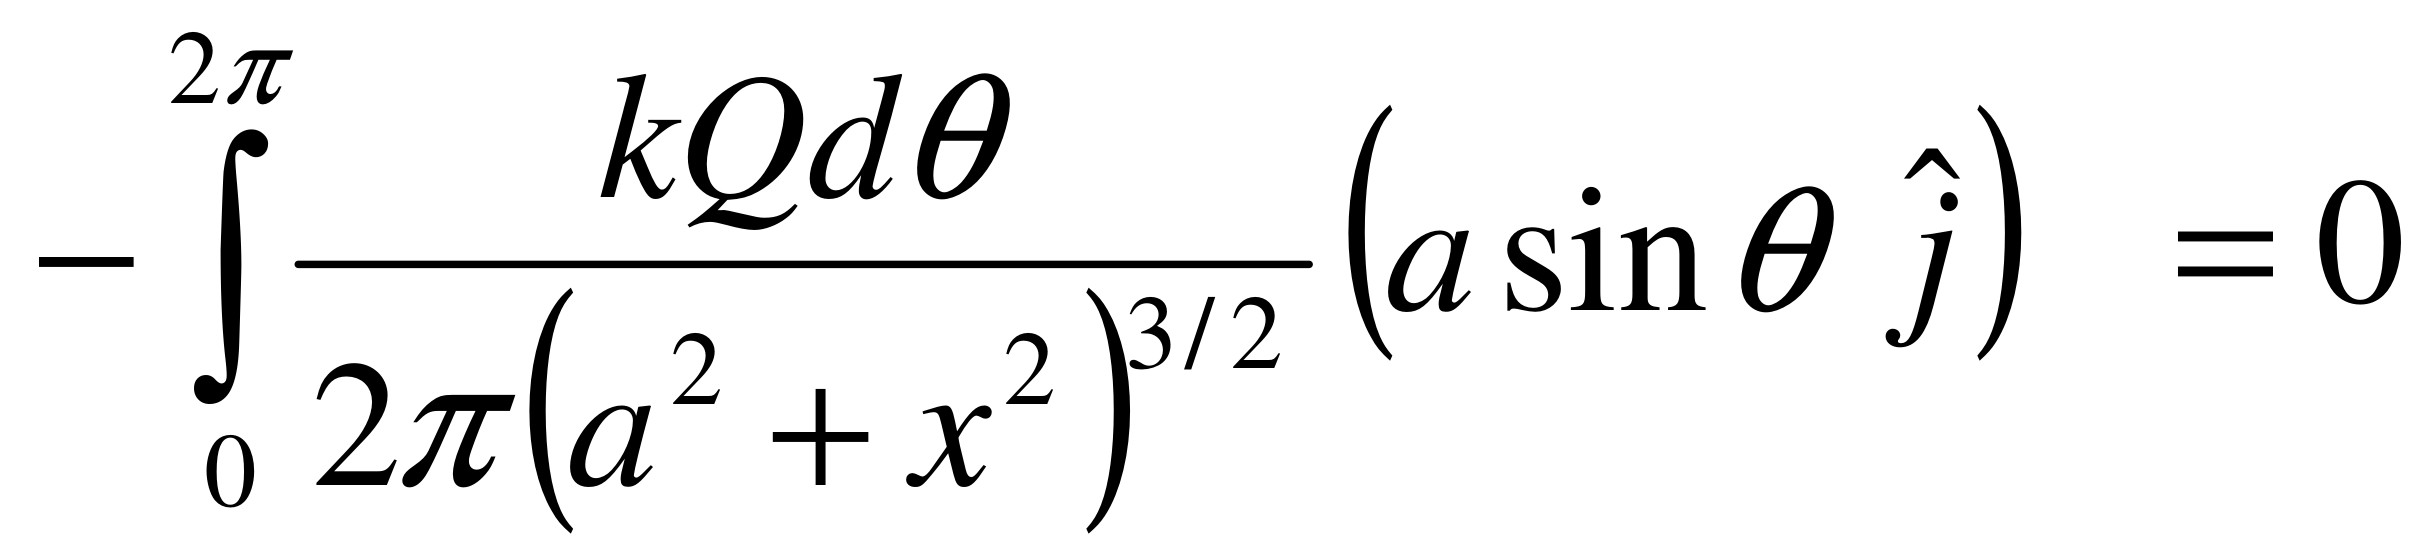
\includegraphics[height=38pt]{wordmath}
\end{frame}

\begin{frame}[fragile]
    \frametitle{Structure of a \LaTeX\ Document}
    \begin{lstlisting}
    *@\tikzmark{T1}@**@\tikzmark{P1}@*\documentclass[12pt]{article}
    \usepackage[margin=25mm]{geometry}*@\tikzmark{P2}@*
    \begin{document}
    *@\tikzmark{B1}@*Hello World from \LaTeX !
    \begin{equation}
      \sum_{n = 0}^\infty {x^n \over n!} = e^x
    \end{equation}*@\tikzmark{B2}@*
    \end{document}
    \end{lstlisting}
    \braced{P1}{P2}{Preamble}
    \braced{B1}{B2}{Body}
    \vspace{-15pt}
    \visible<2>{\begin{block}{Output}
        \justifying
        Hello World from \LaTeX !
        \begin{equation}
            \sum_{n = 0}^\infty \frac{x^n}{n!} = e^x
        \end{equation}
    \end{block}}
\end{frame}

\begin{frame}[fragile]
    \frametitle{Control Sequences}
    \begin{itemize}[<+->]
        \item Immediately after typing `\verb|\|', \TeX\ expects
            a control word or symbol.
        \item A control word constists of a backslash followed by one or more
            \emph{letters}.
        \item A control symbol constists of a backslash followed by a single
            \emph{nonletter}.
        \item Example: `\verb|\input MS|' causes \TeX\ to begin
            reading a file called `\texttt{MS.tex}'.
        \item Example: \TeX\ converts `\verb|George P\'olya and Gabor Szeg\"o|'
            to `George P\'olya and Gabor Szeg\"o.'
        \item A space after a control word is ignored, to fix this, escape
            the space afted a control word when required. \par
            \verb|\TeX\ ignores spaces after control words.|
    \end{itemize}
\end{frame}

\begin{frame}[fragile]
    \frametitle{Grouping}
    %\vspace{-45 pt}
    \hskip-130pt
    \begin{minipage}{\linewidth}
    \begin{Verbatim}[fontsize=\fontsize{100}{120}]
    { }
    \end{Verbatim}
\end{minipage}
\end{frame}

\begin{frame}[fragile]
    \frametitle{Fonts of Type in \LaTeX}
    \verb|\textrm{This}| \textrm{This} produces roman typeface output.\par
    \verb|\textsl{This}| \textsl{This} produces slanted typeface output.\par
    \verb|\textit{This}| \textit{This} produces italics typeface output.\par
    \verb|\textbf{This}| \textbf{This} produces bold typeface output.\par
    \verb|\texttt{This}| \texttt{This} produces typewriter typeface output.\par
    \verb|\textsf{This}| \textsf{This} produces sans typeface output.\par
\end{frame}

\begin{frame}[fragile]
    \frametitle{Installing \TeX\ Live}
    Arch Linux:\break
    \verb|# pacman -S texlive-most|\par
    \medskip
    Debian/Ubuntu/Mint:\break
    \verb|# apt-get install texlive-full|\par
    \medskip
    Fedora:\break
    \verb|# yum install texlive|\par
    \medskip
    Windows/OS X:\break
    Follow instructions at \texttt{http://tug.org}
\end{frame}

\begin{frame}
    \frametitle{Running \TeX}
    \centering
    \includegraphics[width=0.6\linewidth]{/home/jack/Dropbox/g/runningtex}
\end{frame}

\begin{frame}[fragile]
    \frametitle{Running \LaTeX}
    When you start \verb|pdflatex|, you will see the following:

    \begin{verbatim}
    This is pdfTeX, Version 3.14159265-2.6-1.40.16
    (TeX Live 2015) (preloaded format=pdflatex)
    **
    \end{verbatim}

    \pause
    The `\verb|**|' is \TeX's way of asking you for an input filename. If you
    don't want to type in the filename through standard input each time,
    provide the filename as the first argument.

    \pause
    \medskip
    To use \TeX\ in a REPL like manner, type `\verb|\relax|' at the prompt for a
    filename. This is \TeX's NoOp command, in this case you are using it to
    tell \TeX\ to expect nothing after an `\verb|\input|'.

    \pause
    \medskip
    pdf\TeX\ will produce a PDF file.
\end{frame}

\begin{frame}[fragile]
    \frametitle{The \texttt{documentclass}}
    When you start a document, you start it with a line that reads something
    like this:
    \begin{lstlisting}[xleftmargin=0pt]
    \documentclass{article}
    \end{lstlisting}
    \pause
    There are actually many \texttt{documentclass}es to choose from:

    \begin{multicols}{4}
        \begin{itemize}
            \ttfamily
            \item article
            \item IEEEtran
            \item proc
            \item minimal
            \item report
            \item book
            \item memior
            \item letter
            \item exam
            \item leaflet
            \item beamer
            \rmfamily
            \item ...
        \end{itemize}
    \end{multicols}
    \pause
    You can also specify options like this:
    \begin{lstlisting}[xleftmargin=0pt]
    \documentclass[12pt,a4paper,titlepage]{article}
    \end{lstlisting}
\end{frame}

\begin{frame}[fragile]
    \frametitle{Environments}
    \begin{lstlisting}
    *@\tikzmark{T1}@*...
    *@\tikzmark{E1}@*\begin{itemize}
        \item An item
        \item Another item
    \end{itemize}*@\tikzmark{E2}@*
    ...
    \end{lstlisting}
    \braced{E1}{E2}{environment}
    \visible<2>{
        \begin{block}{Output}
            \begin{itemize}
                \item An item
                \item Another item
            \end{itemize}
        \end{block}
    }
\end{frame}

\begin{frame}[fragile]
    \frametitle{Environments}
    \begin{lstlisting}
    *@\tikzmark{T1}@*...
    *@\tikzmark{N1}@*\begin{enumerate}
        \item An item
        \item Another item
    \end{enumerate}*@\tikzmark{N2}@*
    ...
    \end{lstlisting}
    \braced{N1}{N2}{environment}
    \begin{block}{Output}
        \begin{enumerate}
            \item An item
            \item Another item
        \end{enumerate}
    \end{block}
\end{frame}

\lstset{xleftmargin=-10pt}

\begin{frame}[fragile]
    \frametitle{Mathematics in \LaTeX}
    Use the \verb|equation| environment for basic equation displays:
    \begin{lstlisting}
    \begin{equation}
        \lim_{\Delta x \to 0} \frac{f(x + \Delta x) - f(x)}{\Delta x}
    \end{equation}
    \end{lstlisting}
    \pause
    \begin{block}{Output}
        \vskip -5pt
        \begin{equation}
            \lim_{\Delta x\to0} \frac{f(x + \Delta x) - f(x)}{\Delta x}
        \end{equation}
    \end{block}
    \pause
    Or use `\verb|$ ... $|' to quickly show math in a paragraph:
    \begin{lstlisting}
    ... we can see that as $x \to \infty$, the amount of ...
    \end{lstlisting}
    \pause
    \begin{block}{Output}
        ... we can see that as $x \to \infty$, the amount of ...
    \end{block}
\end{frame}


\begin{frame}[fragile]
    \frametitle{How \TeX\ Reads What You Type}
    \begin{itemize}
        \item A $\langle\hbox{return}\rangle$ is like a space
        \pause\item Two spaces in a row count as a single space
        \pause\item A blank line denotes the end of a paragraph
    \end{itemize}

    \pause
    \TeX\ also categorgizes your characters. There are 16 categories as follows:
    \begin{table}
        \tiny
    \begin{tabular}{c l l || c l l}
        \emph{Cat} & \emph{Meaning} & \emph{Default} & \emph{Cat} & \emph{Meaning} & \emph{Default} \\
        \hline
        0 & Escape character & \verb|\| & 8 & Subscript & \verb|_| \\
        1 & Begin group      & \verb|{| & 9 & Ignored characer & $\langle\hbox{null}\rangle$ \\
        2 & End group        & \verb|}| & 10 & Space           & $\langle\hbox{space}\rangle$ \\
        3 & Math shift       & \verb|$| & 11 & Letter          & \verb|A-Z|,\verb|a-z| \\
        4 & Alignment tab    & \verb|&| & 12 & Other character & \\
        5 & End of line      & $\langle\hbox{return}\rangle$ & 13 & Active character & \verb|~| \\
        6 & Parameter        & \verb|#| & 14 & Comment character & \verb|%| \\
        7 & Superscript      & \verb|^| & 15 & Invalid character & $\langle\hbox{delete}\rangle$ \\
    \end{tabular}
    \end{table}
    Don't worry too much about this. All this means is that you will have to
    escape a few special characters.
\end{frame}

\begin{frame}
    \frametitle{Line Breaking}
    \begin{itemize}[<+->]
        \item \TeX\ has a badness value from 0 to 10,000, where 0 is perfect
            and 10,000 is infinitely bad, for almost everything in your document
            that is flexible.
        \item When a line is perfect in spacing between words and no
            hyphenation, the badness will be zero.
        \item As words get too tight or too narrow, the badness increases.
        \item Hyphenation in words adds a lot of badness!
        \item \TeX\ then optimises the badness of each line, trying to get it
            as low as possible.
    \end{itemize}
\end{frame}

\begin{frame}[fragile]
    \frametitle{Sectioning}
    Use the commands:
    \begin{lstlisting}
    \part{Part I}               % only in the book class
    \chapter{Awesome Chapter}   % only in book, report
    \section{Optimal Awesome}
    \subsection{Here It Is}
    \end{lstlisting}

    \pause
    Then you can generate your table of contents using:
    \begin{lstlisting}
    \tableofcontents
    \end{lstlisting}
\end{frame}

\begin{frame}[fragile]
    \frametitle{Graphics}
    In your preamble, include the \verb|graphicx| package:
    \begin{lstlisting}
    \usepackage{graphicx}
    \end{lstlisting}
    Then in your body: (arguments and file extension optional)
    \begin{lstlisting}
    \includegraphics[width=4cm]{coolpix.png}
    \end{lstlisting}
\end{frame}

\begin{frame}[fragile]
    \frametitle{Tables}
    `\verb|&|' acts as an alignment character in the \verb|tabular|
    environment, `\verb|\\|' acts as a newline:
    \begin{lstlisting}
    \begin{tabular}{ |l|l| }
        \hline
        stuff & stuff \\ \hline
        stuff & stuff \\
        \hline
    \end{tabular}
    \end{lstlisting}
    \pause
    \begin{block}{Output}
        \begin{tabular}{ |l|l| }
            \hline
            stuff & stuff \\ \hline
            stuff & stuff \\
            \hline
        \end{tabular}
    \end{block}
    \pause
    Also take a look at the excellent \texttt{tabu} package.
\end{frame}

\begin{frame}[fragile]
    \frametitle{Automagically Numbered Floating Figures and Tables}
    \begin{lstlisting}
    \begin{figure}
        \centering
        \includegraphics[width=4cm]{coolpix}
        \caption{This is a really cool picture}
    \end{figure}
    \end{lstlisting}
    \pause

    \begin{lstlisting}
    \begin{table}
        \centering
        \caption{Important Data About Stuff}
        \begin{tabular}{ | l | l | c | }
            ...
        \end{tabular}
    \end{table}
    \end{lstlisting}
    \pause

    You can also generate a List of Figures and a List of Tables:
    \begin{lstlisting}
    \listoffigures
    \listoftables
    \end{lstlisting}
\end{frame}

\begin{frame}[fragile]
    \frametitle{Presentations}
    Use the \texttt{beamer} class, slides are in the \texttt{frame}
    environment.
    \begin{lstlisting}
    \documentclass{beamer}
    \begin{document}
    \begin{frame}
        \frametitle{Relevant Title}
        Hello World!
        \pause % Advance slide to continue
        This won't show till you click.
        \begin{block}{Cool Information}
            This shows in a fancy blue block
        \end{block}
    \end{frame}
    \end{document}
    \end{lstlisting}
\end{frame}

\begin{frame}
    \sffamily
    \frametitle{\sffamily Relevant Title}
    Hello World!
    \pause
    This won't show till you click.
    \begin{block}{\sffamily Cool Information}
        This shows in a fancy blue block
    \end{block}
\end{frame}

\begin{frame}[fragile]
    \frametitle{Cool Tricks}
    \centering
    Using Ti$k$Z...

    \hskip 110pt 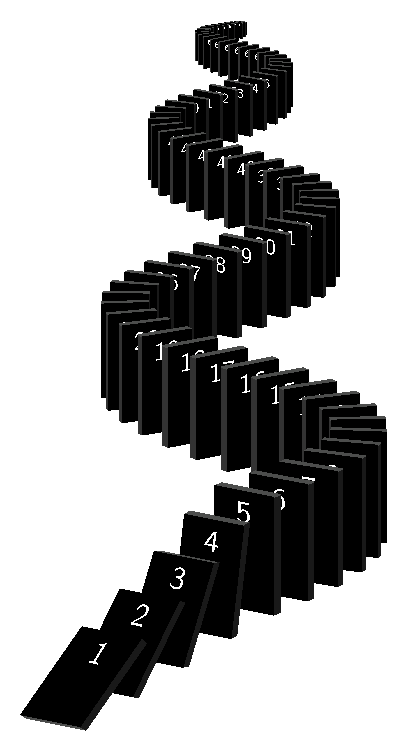
\includegraphics[height=0.6\paperheight]{dominoes.pdf}
\end{frame}

\begin{frame}
    \frametitle{Comprehensive \TeX\ Archive Network (CTAN)}
    \begin{wrapfigure}{r}{0pt}
        
\includegraphics[width=4cm]{ctan}
    \end{wrapfigure}
    CTAN is a great site that has all of the \TeX\ and \LaTeX\ packages and
    sources.

    \texttt{http://ctan.org}
\end{frame}

\begin{frame}
    \frametitle{Resources and Recommended Reading}
    \begin{itemize}[<+->]
        \item The \TeX book, Donald E. Knuth
        \item \LaTeX: A Document Preparation System, Leslie Lamport
        \item The \LaTeX\ Companion, Frank Mittelbach \& Michel Goossens
        \item The \LaTeX\ Book on Wikibooks
        \item \texttt{http://texdoc.net}
        \item \TeX\ Users Group: \texttt{http://tug.org}
    \end{itemize}
\end{frame}

\begin{frame}
    \frametitle{Getting Help}
    \only<1>{
        \centering
        
\includegraphics[width=0.9\linewidth]{conTeXt-help}
    }
    \only<2>{
        You likely haven't found a bug in \TeX. Knuth pays \texttt{0x\$80.00}
        for every bug found in the current stable versions of \TeX\ and \MF.
        \begin{itemize}
            \item \TeX\ Stack Exchange
            \item \texttt{texhax} mailing list
            \item Come to LUG!
        \end{itemize}
    }
\end{frame}

\end{document}
